\definecolor{accent}{HTML}{1F5C99}
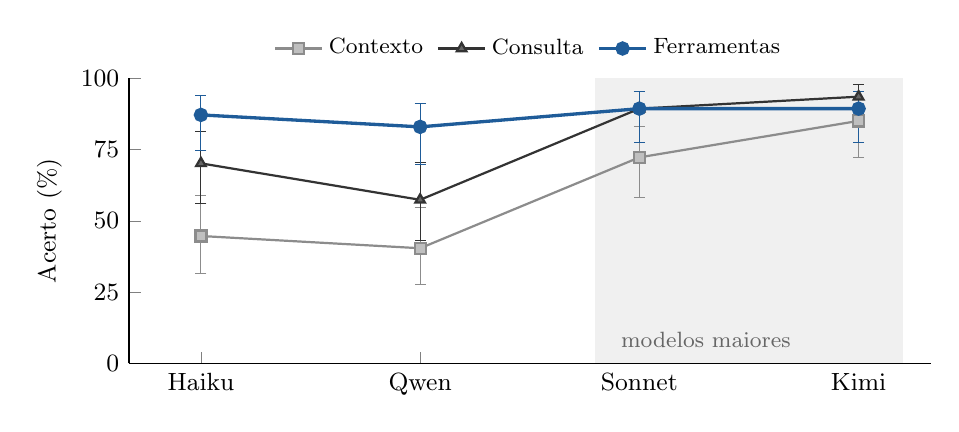
\begin{tikzpicture}
\begin{axis}[
  width=0.97\columnwidth, height=5.2cm, ymin=0, ymax=100, clip=false,
  symbolic x coords={Haiku,Qwen,Sonnet,Kimi}, xtick=data, enlarge x limits={abs=26pt},
  ylabel={Acerto (\%)}, ytick={0,25,50,75,100}, axis x line*=bottom, axis y line*=left,
  tick label style={font=\small}, label style={font=\small}, legend style={font=\footnotesize, draw=none,
  fill=none, at={(0.5,1.03)}, anchor=south, legend columns=-1,
  /tikz/every even column/.append style={column sep=3pt}},
  error bars/y dir=both, error bars/y explicit, error bars/error bar style={line width=0.4pt},
]
\fill[black!6] ([xshift=-16pt]axis cs:Sonnet,0) rectangle ([xshift=16pt]axis cs:Kimi,100);
\node[font=\footnotesize, black!60, anchor=south] at ([xshift=24pt]axis cs:Sonnet,2) {modelos maiores};
\addplot[black!45, thick, mark=square*, mark options={fill=black!25}] coordinates {(Haiku,44.7) += (0,14.1) -= (0,13.3) (Qwen,40.4) += (0,14.2) -= (0,12.8) (Sonnet,72.3) += (0,10.7) -= (0,14.1) (Kimi,85.1) += (0,7.5) -= (0,12.8)};
\addplot[black!80, thick, mark=triangle*, mark options={fill=black!60}] coordinates {(Haiku,70.2) += (0,11.1) -= (0,14.2) (Qwen,57.4) += (0,13.0) -= (0,14.2) (Sonnet,89.4) += (0,6.0) -= (0,12.0) (Kimi,93.6) += (0,4.2) -= (0,10.8)};
\addplot[accent, very thick, mark=*] coordinates {(Haiku,87.2) += (0,6.8) -= (0,12.4) (Qwen,83.0) += (0,8.1) -= (0,13.1) (Sonnet,89.4) += (0,6.0) -= (0,12.0) (Kimi,89.4) += (0,6.0) -= (0,12.0)};
\legend{Contexto,Consulta,Ferramentas}
\end{axis}
\end{tikzpicture}
